% TFG - José Ángel Martín Baos. Escuela Superior de Informática. 2018
% !TeX spellcheck = en_GB

%%%% CHAPTER: Results %%%
\chapter{Results} % TODO
\label{chap:results}

\drop{I}{n} this chapter, the different results obtained during the development of this \ac{BSc.} thesis are presented. The working methodology presented in Chapter \ref{chap:methodology} is used to carry out the work. In first place, the initial Sprint is presented, where the Scrum team is set up, as well as the initial planning of the project. Subsequently, the different Sprints are presented, where the work planned in the initial Sprint are carried out.




%%% Sprint 0
\section{Sprint 0: Initial planning}
\label{Section:Sprint0}
In this first phase, the main objective is to define the Scrum team, the user stories, the project plan and the temporal and cost planning. Then, the draft (“Anteproyecto”) have to be written. Once this Sprint was completed, the project started  as it was stated in the temporal planning. The task associated to this initial Sprint is shown in Table \ref{tab:Sprint0-Tasks}.

\begin{table}[hp]
	\centering
	{\small
		\begin{tabular}{|p{.5\textwidth}P{.14\textwidth}|}
	\hline
	\rowcolor{tabheadbg}
	\multicolumn{2}{|c|}{\textscale{.8}{\textbf{Sprint 0 tasks}}} \\
	\hline
	\hline
	\textscale{.8}{\textbf{Task}} 			& \textscale{.8}{\textbf{Estimation (h)}} \\
	\hline
	Define the Scrum team					& 0.5 \\
	\hline
	Investigate about similar proposals		& 6 \\
	\hline
	Define the user stories					& 5 \\
	\hline
	Generate the project plan				& 3 \\
	\hline
	Generate the temporal planning			& 3 \\
	\hline
	Generate the cost planning				& 2 \\
	\hline
	Create a GitHub repository				& 0.5 \\
	\hline
	Write the draft (“Anteproyecto”)		& 15 \\
	
	\Xhline{3\arrayrulewidth}
	\textbf{Total} 							& \textbf{35} \\
	\hline

\end{tabular}
	}
	\caption{Sprint 0 tasks}
	\label{tab:Sprint0-Tasks}
\end{table}

\subsection{Scrum Team}
Following the scrum roles defined in Section \ref{5-ScrumTeam}, the Scrum team have the following structure:
\begin{itemize}
	\item \textbf{Product Owner:} Ricardo García Ródenas
	\item \textbf{Scrum Master:} Luis Rodríguez Benítez
	\item \textbf{Development Team:} José Ángel Martín Baos
\end{itemize}

\subsection{Product Backlog}
The Scrum Team had several meetings after the completion of the draft (“Anteproyecto”) and the different requirements stated in the draft were translated to user stories that should be accomplished during the execution of the BSc. thesis. The Scrum Team has defined the different user stories, as well as the priority and the estimated duration they will have using planning poker technique. In this technique, the product owner explains an user story and each member of the development team writes his estimation into a card \cite{Gar18}. Nonetheless, in this case, all the members of the Scrum Team have participated in the estimation. The final list of User stories is shown in Table \ref{tab:User-Stories}.

\begin{table}[hp]
	\centering
	{\small
		\begin{tabular}{ |P{.08\textwidth}p{.56\textwidth}P{.1\textwidth}P{.08\textwidth}|}
	\hline
	\rowcolor{tabheadbg}
	\multicolumn{4}{|c|}{\textscale{.8}{\textbf{User stories}}} \\
	\hline
	\textscale{.8}{\textbf{ID}}	& \textscale{.8}{\textbf{User history}}	& \textscale{.8}{\textbf{Priority}}	& \textscale{.8}{\textbf{Estimate}} \\
	\hline
	1 	& Configure Raspberry Pi Architecture 						& High 	& \REDNOTE{15}h \\ 
	\hline
	2 	& Install PiCamera into Raspberry Pi 						& High 	& \REDNOTE{5}h \\ 
	\hline
	3 	& Calculate the vehicle flow		 						& High 	& \REDNOTE{30}h \\ 
	\hline
	4 	& Install environmental and gas sensors into Raspberry Pi	& High 	& \REDNOTE{25}h \\ 
	\hline
	5 	& Obtain and process data from the sensors					& High 	& \REDNOTE{30}h \\ 
	\hline	

\end{tabular}
	}
	\caption{User stories}
	\label{tab:User-Stories}
\end{table}
	
The different user stories are presented in its corresponding Sprint. Each user story is composed by the following fields:
\begin{itemize}
	\item \emlst{Sprint.} It indicates the Sprint number to which the user story belongs to.
	\item \emlst{Priority.} Priority given to the user story. It can take the levels: low, medium and high.
	\item \emlst{Effort.} The estimated duration of the user story in hours. 
	\item \emlst{Name.} The label of the user story.
	\item \emlst{Description.} It is a brief definition of the user story.
	\item \emlst{Tasks.} It consists of a list of the different tasks that must be executed to complete the user story.
	\item \emlst{Tests.} It is a list of the different tests defined specifically for the user story.
\end{itemize}

\subsection{Project plan}
Once the different user stories have been defined, the next step is to define the different Sprints that must be carried out and their associated user stories (Table \ref{tab:Sprints}). This is only the initial plan of the project, so that means that additional tasks can be created to solve errors or to add functionalities not taken into account in this initial phase of the project.

\begin{table}[hp]
	\centering
	{\small
		\begin{tabular}{|P{.08\textwidth}p{.56\textwidth}P{.15\textwidth}P{.08\textwidth}|}
	\hline
	\rowcolor{tabheadbg}
	\multicolumn{4}{|c|}{\textscale{.8}{\textbf{Sprints}}} \\
	\hline
	\hline
	\textscale{.8}{\textbf{Sprint}}			& \textscale{.8}{\textbf{Name}}	& \textscale{.8}{\textbf{User stories}}	& \textscale{.8}{\textbf{Estimate}} \\
	\hline
	0 	& Initial planning		 	& - 	& 35h \\ 
	\hline
	1 	& Development a basic algorithm to calculate the flow of vehicles		 		 	& 1, 2, 3 	& 50h \\ 
	\hline
	2 	& Design of an environmental parameters monitoring system		 	& \REDNOTE{...} 	& \REDNOTE{X}h \\ 
	\hline

\end{tabular}
	}
	\caption{Sprints}
	\label{tab:Sprints}
\end{table}

\subsection{Temporal planning}
Considering Table \ref{tab:Sprints}, the temporal planning for this BSc. thesis is defined. The total duration of the project when all the Sprints finish is estimated to be 225 hours. The project started on 18th September 2017 and was planned to be finished on 18th June 2018. Therefore, this means that the student has dedicated 6.25 hours per week in the project. Taking all these elements into account the Gantt diagram shown in Figure \ref{fig:6-Gantt} was defined.

\begin{figure}[!h]
	\begin{center}
		\begin{ganttchart}[%Specs
			x unit = 9pt,
			vgrid={*{3}{draw=none},dotted},
			title/.style={fill=gray!30, draw=black, very thick},
			canvas/.style={fill=gray!10, draw=black, dashed, very thick},
			bar/.style={fill=barblue, draw=black},
			link/.append style={thick}
			]{1}{40}
			\gantttitle{2017}{16}
			\gantttitle{2018}{24} \\
			\gantttitle{Sep}{4}
			\gantttitle{Oct}{4}
			\gantttitle{Nov}{4}
			\gantttitle{Dec}{4}
			\gantttitle{Jan}{4}                      
			\gantttitle{Feb}{4}
			\gantttitle{Mar}{4}
			\gantttitle{Apr}{4}
			\gantttitle{May}{4}
			\gantttitle{Jun}{4}\\
			
			% Draft (“Anteproyecto”)
			\ganttgroup{Draft}{3}{8} \\
			\Dganttbar{Sprint 0}{35h}{3}{8} \\	
			
			% Draft (“Anteproyecto”)
			\ganttgroup{BSc. Thesis}{9}{38} \\
			\Dganttbar{Sprint 1}{50h}{9}{16} \\
			\Dganttbar{Sprint 2}{55h}{17}{24} \\
			\Dganttbar{Sprint 3}{35h}{25}{30} \\
			\Dganttbar{Sprint 4}{50h}{31}{38}
			\ganttlink[link type=rdldr*, link bulge 2=9, link mid=0.25]{elem5}{elem9}
			\ganttlink[link bulge=1]{elem7}{elem9}
			\ganttlink[link bulge=1]{elem9}{elem11}
		\end{ganttchart}
		\caption{Temporal planning}
		\label{fig:6-Gantt}
	\end{center}
\end{figure}

\subsection{Cost planning}
To manage the costs for the development of this project, two tables had been elaborated. Table \ref{tab:Hardware-Costs} indicates the costs related to the hardware resources that might be purchased in order to execute the project. Moreover, some development costs must be taken into account, as it is indicated in Table \ref{tab:Development-Costs}. For the purpose of calculating the salary of the developer, the \ac{UCLM} retributions table of labor contracts for research projects on 2017 has been used. Therefore, it has been considered that the developer will have a “Tercera-O-II” category, meaning that the annual cost of a full-time job is $23.025.67$\euro{}. Taking into account that a full-time job in the UCLM consist of 7 work hours per day and 225 working days per year then, the Table \ref{tab:Development-Costs} is obtained. 

Taking into account Tables \ref{tab:Hardware-Costs} and \ref{tab:Development-Costs}, an estimation of the total cost of the project can be $3685.87$\euro{}.

\begin{table}[hp]
	\centering
	{\small
		\begin{tabular}{ |p{.5\textwidth}P{.1\textwidth}r|}
	\hline
	\rowcolor{tabheadbg}
	\multicolumn{3}{|c|}{\textscale{.8}{\textbf{Hardware costs}}} \\
	\hline
	\hline
	\textscale{.8}{\textbf{Item}}	& \textscale{.8}{\textbf{Quantity}}	& \textscale{.8}{\textbf{Cost}} \\
	\hline
	Raspberry Pi 3 					& 2 	& 49\euro{} \\ 
	\hline
	Pi NoIR Camera V2 				& 2 	& 28\euro{} \\ 
	\hline
	Memory card Samsung SDHC
	EVO 8gb Class 10+ 				& 2		& 8\euro{} \\ 
	\hline
	Power bank battery 				& 2 	& 29\euro{} \\ 
	\hline
	Camera Case		 				& 2 	& 14\euro{} \\ 
	\hline
	Raspberry Pi Sense HAT			& 2 	& 42\euro{} \\ 
	\hline
	Stacking Header 40 PIN 			& 2 	& 7\euro{} \\ 
	\hline
	MQ7 Gas Sensor		 			& 2 	& 2.5\euro{} \\ 
	\hline
	MQ2 Gas Sensor 					& 2 	& 3\euro{} \\ 
	\hline
	MCP3008 AD Conversor			& 2 	& 9\euro{} \\ 
	\hline
	Prototype shield  				& 1 	& 1.5\euro{} \\ 
	\hline
	Wires 							& 1 	& 7\euro{} \\ 
	\hline
	LM317 							& 2 	& 1.75\euro{} \\ 
	
	\Xhline{2\arrayrulewidth}
	\textbf{TOTAL:} &  		& \textbf{395\euro{}} \\ 
	\hline

\end{tabular}

	}
	\caption{Hardware investments}
	\label{tab:Hardware-Costs}
\end{table}

\begin{table}[hp]
	\centering
	{\small
		\begin{tabular}{ |p{.1\textwidth}P{.1\textwidth}r|}
	\hline
	\rowcolor{tabheadbg}
	\multicolumn{3}{|c|}{\textscale{.8}{\textbf{Development costs}}} \\
	\hline
	\hline
	\textscale{.8}{\textbf{Sprint}}	& \textscale{.8}{\textbf{Hours}}	& \textscale{.8}{\textbf{Cost}} \\
	\hline
	0			& 35h 			& \REDNOTE{X}\euro{} \\ 
	\hline
	\REDNOTE{XXX}	& \REDNOTE{X}h 		& \REDNOTE{X}\euro{} \\ 
	
	
	\Xhline{2\arrayrulewidth}
	\textbf{TOTAL:} & \textbf{\REDNOTE{X}h} 		& \textbf{\REDNOTE{X}\euro{}} \\ 
	\hline

\end{tabular}
	}
	\caption{Development costs}
	\label{tab:Development-Costs}
\end{table}


\newpage
%%% Sprint 1
\section{Sprint 1: Development of an algorithm to calculate the traffic flows based on video data}
\label{Section:Sprint1}
According to the project plan, in this Sprint, the tasks associated to the user stories 1, 2 and 3 should be executed. This iteration aims to obtain an algorithm to count the number of vehicles that cross a street in a certain amount of time so as to obtain the vehicle flow. To be able to count the number of vehicles using the PiCamera, \emword{motion vectors} are used. Therefore, some research about video codification and \emword{motion vectors} is needed before implementing the algorithm. But first, it is necessary to configure the Raspberry Pi architecture and to install the PiCamera. 

During the planning meeting, the different user stories addressed in this Sprint has been analysed. Consequently, they have been divided into several tasks and tests. The three user stories are shown in Tables from \ref{tab:Sprint1-User-story-1} to \ref{tab:Sprint1-User-story-3}.

\UserStoryTable{1}{1}{High}{15}
{Configure Raspberry Pi Architecture}
{Raspbian \ac{OS} and all the components must be installed and configured.}
{	\item Install and configure Raspbian \ac{OS}.
	\item Install the necessary libraries.
}{	\item Check if the system works correctly using a SSH connection.
	\item Check if python works.
}

\UserStoryTable{2}{1}{High}{5}
{Install PiCamera module in the Raspberry Pi}
{The PiCamera module must be working and some sample videos should be recorded in order to check the camera.}
{	\item Install the PiCamera module.
	\item Develop a program to record videos.
}{	\item Check if the camera is working correctly by storing some photos and videos.
}

\UserStoryTable{3}{1}{High}{30}
{Develop an algorithm to calculate the vehicle flow}
{Development of an algorithm that counts the number of vehicles travelling on a street and determines their direction.}
{	\item Extract the \emword{motion vectors} while recording a video with the PiCamera module using PiMotionAnalysis.
	\item Read and process the data stored containing the \emword{motion vectors}.
	\item Develop a noise filter using moving averages.
	\item Develop the algorithm to count vehicles.
}{	\item Check the correctness of the \emword{motion vectors} extracted.
	\item Compare the data before and after applying the noise filter.
	\item Assess the performance of the traffic-counting algorithm.
}

\subsubsection{T1.1.1. Install and configure Raspbian \ac{OS}}
The first step consist of the Raspbian \ac{OS} installation and its configuration. The Operating System allows us not only to execute programs into the Raspberry Pi device, but also to connect it to the network, which is necessary to send the data collected.

\subsubsection{T1.1.2. Install the necessary libraries}
When the \ac{OS} is installed, some libraries need to be installed in order to execute the programs that are developed in the following Sprints. All these steps are detailed in the Appendix \ref{chap:installation_guide}. Once installed, the functionality of the system has been checked using a SSH connection from the development computer to the Raspberry, in order to ease the access to the system. 

\subsubsection{T1.2.1. Install the PiCamera module}
The next step is connecting the PiCamera module and configuring it as it is detailed in Appendix \ref{chap:installation_guide}. Now, the device is the one shown in Figure \ref{fig:6-Sistema_v1}. 

\begin{figure}[!h]
	\begin{center}
		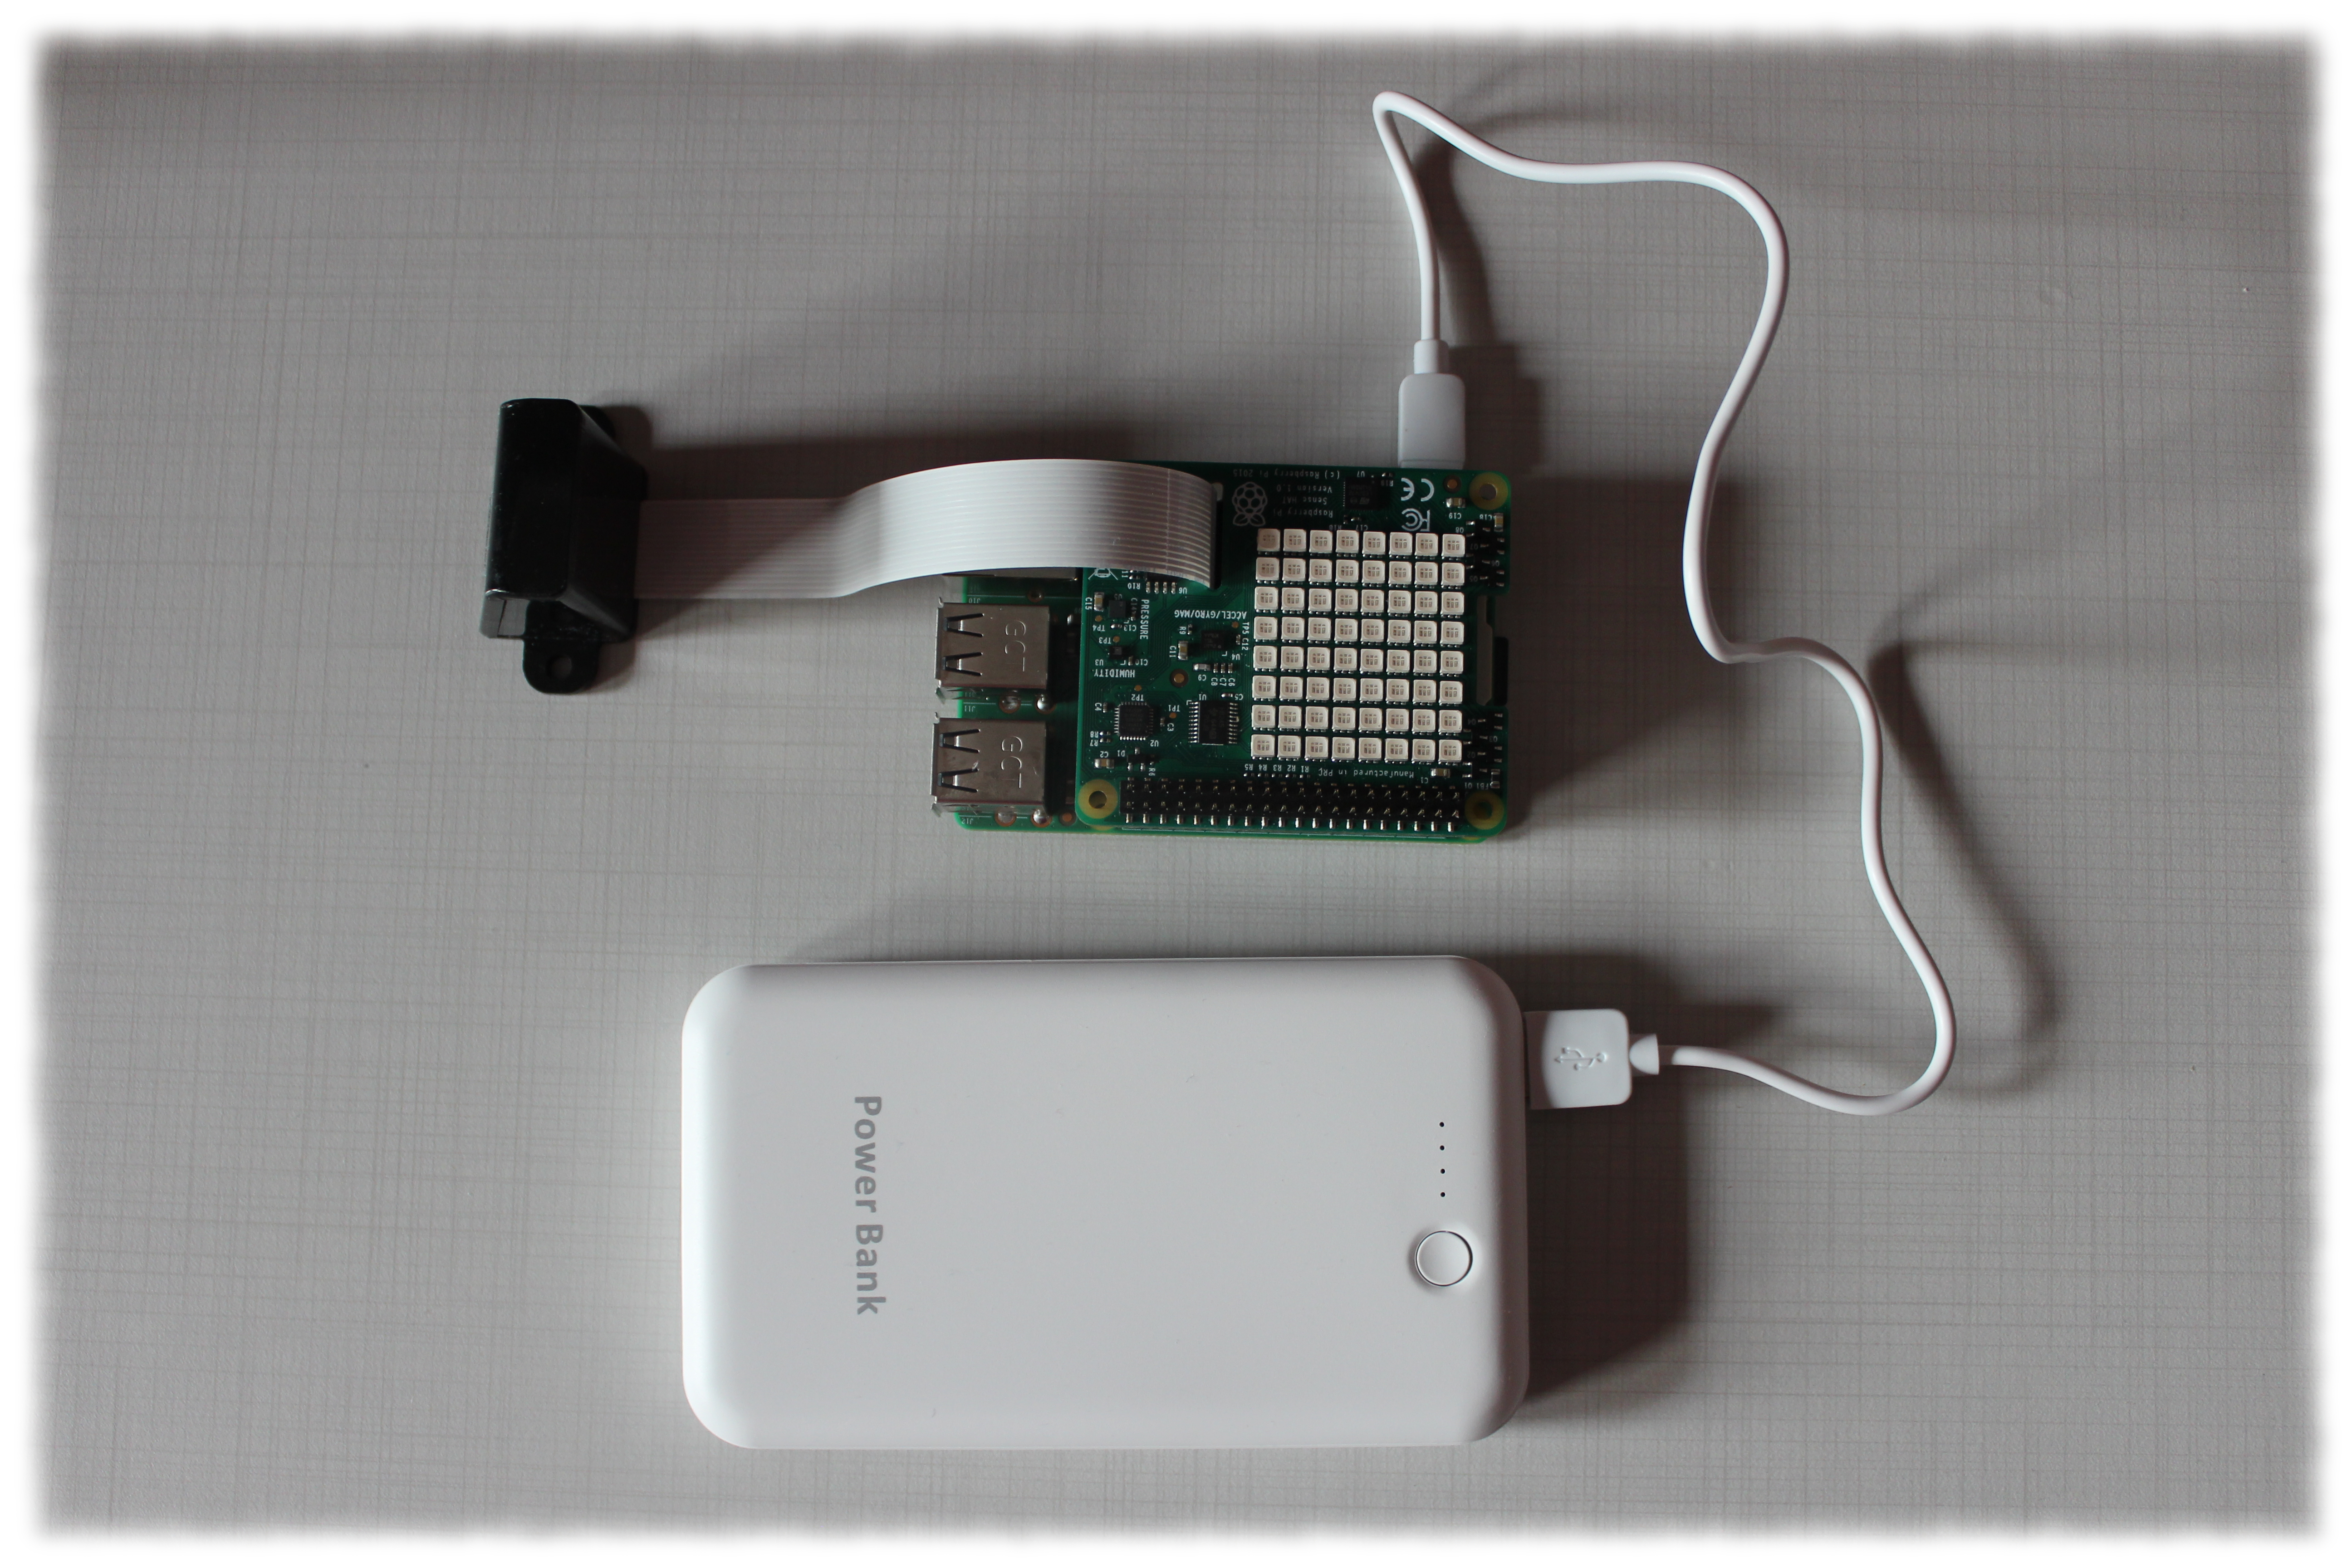
\includegraphics[width=0.8\textwidth]{6-Sistema_v1.jpg}
		\caption{Device structure with PiCamera installed}
		\label{fig:6-Sistema_v1}
	\end{center}
\end{figure}

\subsubsection{T1.2.2. Develop a program to record videos}
A configuration file has been implemented containing some variables that are used by several modules of the device. Hence, these values are stored only once and can be changed without difficulties. The file format is shown and explained in Appendix \ref{chap:user_manual}. The parameters related to the camera are shown in Listing \ref{lst:6-camera-config}.

\lstinputlisting[language=Python, firstline=4, texcl, caption = {Part of \texttt{config.py} file containing the camera parameters}, label = lst:6-camera-config]{code/6-camera-config.py}

To ensure the correct functionality of the camera, a set of test videos are recorded. For that purpose and following the examples provided in PiCamera documentation \cite{PiCameraDoc}, a script has been developed. This script is shown in Listing \ref{lst:6-camera-video-recording}, and when it is executed it must wait two seconds to ensure the camera is correctly initialized. Then the camera starts recording during 60 seconds (as it is defined in \texttt{config.py}) and finally the video is saved in the file \texttt{my\_video.h264} in h264 video format.

\lstinputlisting[language=Python, firstline=4, texcl, caption = {Video recording with PiCamera script}, label = lst:6-camera-video-recording]{code/6-camera-video-recording.py}

\subsubsection{T1.3.1. Extract the \emword{motion vectors} while recording a video with the PiCamera module using PiMotionAnalysis}
\BLUENOTE{The result of the previous task allows to record videos using the PiCamera. Moreover, the PiCamera is capable of generating the motion vector estimates that the camera's H.264 encoder calculates while generating the compressed video. If we suppose a video where each frame has $x$ pixels width and $y$ pixels height, the total number of pixels can be calculated as $ Npx = x\cdot y $. Then, taking into account that each macroblock has a size of $16\times16$ pixels, the number of motion vectors can be calculated in the following way:
$ Nmv = \frac { x }{ 16 } \cdot \frac { y }{ 16 } =\frac { xy }{ 256 } $. 
Hence, we can calculate the percentage of the video information processed using motion vectors instead of pixels as
$ \frac { Nmv }{ Npx } \simeq 0.4\% $. In consequence, we can say that motion vectors are very useful because using them only the 0.4\% of the video information is needed approximately, which makes it a very good approach if low resources are available. }

This task deals with the need of extracting motion data from videos. To achieve this task, \texttt{PiMotionAnalysis} class from \texttt{picamera.array} is used. While recording is in progress, the incoming motion data is stored into a numpy array and the \texttt{analyse} method from this class is called with the resulting array passed as argument \cite{PiCameraDoc}. This class can be extended and then, the \texttt{analyse} method can be overridden. Therefore, in this method, the \emword{motion vectors} can be used to identify motion fields in the video.

The \texttt{analyse} method is called by the camera each time a frame is recorded and the motion vectors obtained for that frame are passed as argument to this method. Then, the algorithm to count the number of vehicles should be implemented inside this method, in order to be executed in each frame. Nonetheless, due to the fact that the camera is configured to record 30 frames per second (fps), the execution of the algorithm should not last more than $1/30$ seconds or even less due to the overhead of the picamera itself when generating the image. This is a major limitation that must be taken into account when designing and implementing the algorithm.

\subsubsection{T1.3.2. Read and process the data stored containing the motion vectors.}
\BLUENOTE{Due to the fact that \texttt{PiMotionAnalysis} class is used when the video is being recorded, it is used in the final implementation but first, in order to complete the different test, \texttt{PiMotionArray} class is used instead. This class converts the incoming motion data into a numpy array as the realtime version (\texttt{PiMotionAnalysis}), but the conversion is made when the recording has finished. This will allow us to have the videos with the motion data stored into files and use them at any time, allowing us to check the implemented algorithm and the different parameters. The class generates a 3-dimensional numpy array organized as (frames, rows, columns) where rows and columns are the number of the rows and columns of the macro-block (see Section \ref{subsect:Macroblocks}) in the frame. In the implementation of this class there is an extra column in the motion vector data that is not going to be used.}

The class used for recording the videos and store the \emword{motion vectors} that have been used later for developing the algorithm to count vehicles is shown in Listing \ref{lst:6-Recorder-Sprint1}. Some parameters are given as arguments: \texttt{distance} and \texttt{angle}. They are used only for the filename so as to know afterwards the conditions of the camera when the video was recorded. In this class, the camera is configured according to the values stored in \texttt{config.py}. When the video had been recorded, it will be stored in a file with extension \texttt{.h264}, as well as the motion data, that will be stored in a file with the same name but with \texttt{.data} extension. To finish with, the video will be also converted to \texttt{.mp4} to ease its view in the development computer. 

\lstinputlisting[language=Python, firstline=4, texcl, caption = {Class used to record a video and its corresponding motion data}, label = lst:6-Recorder-Sprint1]{code/6-Recorder-Sprint1.py}


\subsubsection{T1.3.3. Develop a noise filter using moving averages}
There are some factors that can affect the number of \emword{motion vectors} in a certain frame. Some of these factors can be the incorrect codification of that frame, a small object crossing the image (e.g., a person or an animal) or just light reflection. Moreover, when H.264 video coding is used, there are several types of frames: I-frames, P-frames and B-frames as explained in Section \ref{subsect:H.264}. I-frames do not require other video frames to be decoded, therefore, they do not generate any \emword{motion vectors}. Thus, the number of \emword{motion vectors} in some frames is not going to be close to the reality, causing noise. To solve this problem, a smoothing technique is used. More concretely, simple moving averages calculation is applied.

A simple moving average \cite{Smi15} is an unweighted average of $k$ prior values. Since a time series can be regarded as a sequence of values, $\{x_{t}\}$, being $t=1,2,3,4,…n$, the moving average of these values $\{\overline {x_{t}}\}$ can be computed. If we assume that $n$ is quite large, and we select an integer $k$ which is much smaller than $n$, we can compute the simple moving averages (of order $k$) as shown in Equation (\ref{eq:simple_moving_averages}).

\begin{equation} \label{eq:simple_moving_averages}
\overline { { x }_{ t } } =\frac { 1 }{ k } \sum _{ i=t-k+1 }^{ t }{ { x }_{ i } } ,\quad 2\le k\le n
\end{equation}

The result of applying the simple moving average over the data recorded previously is shown in Figure \ref{fig:6-moving_averages}, where it can be appreciated how the graphic corresponding with the data before applying simple moving averages (black line) has some noise and sometimes it falls to 0. Additionally, it can be observed how the noise is decreased using this smoothing technique (red line).

\begin{figure}[!h]
	\begin{center}
		\includegraphics[width=1\textwidth]{6-moving_averages.pdf}
		\caption{Result of applying moving averages of order $k = 6$ to smooth the data}
		\label{fig:6-moving_averages}
	\end{center}
\end{figure}


\subsubsection{T1.3.4. Develop the algorithm to count vehicles}
To count the vehicles that travels on a street depending on its direction and using the motion data previously stored, an algorithm has been developed. Its pseudocode is shown in Algorithm \ref{alg:count_vehicles_V1}. This algorithm discriminates the vehicles direction (left or right). For each of the directions, the following algorithm is executed: 

\BLUENOTE{For each frame, the number of \emword{motion vectors} in that frame is compared with the number of vectors in the previous frame, increasing or decreasing a variable called \variable{growth}. Once the number of frames exceed the \variable{HEIGHT\_THRESHOLD} variable, if the \variable{growth} variable is positive, the variable \variable{n\_positive\_frames} is increased by one. If this last variable overtakes the \variable{WIDTH\_THRESHOLD} variable, then it can be considererd that a new car has been detected. If the \variable{growth} variable gets equal to \variable{-GROWTH\_LIMIT}, then it is considered that the car has already passed, and the variable \variable{n\_positive\_frames} is restored to its initial value (zero).}

An example of the execution fo the algorithm can be shown in Figure \ref{fig:6-Count_cars_graphic}, where the blue line represents the number of \emword{motion vectors} with left \GREENNOTE{direction} for each frame, and the red line represents the same but for those that go from left to right. The black line, represent the \variable{HEIGHT\_THRESHOLD} variable. Therefore, a car can be predicted if the number of frames in one direction overtakes the \variable{HEIGHT\_THRESHOLD} variable during more than \variable{WIDTH\_THRESHOLD} frames. And, it can be considered that the car has already passed if the number of frames has been decreasing $\variable{GROWTH\_LIMIT} \times 2 $ frames, regardless if the number of \emword{motion vectors} is under the \variable{HEIGHT\_THRESHOLD} variable or not. Therefore, in Figure \ref{fig:6-Count_cars_graphic}, it can be considered that two different vehicles have passed near the frame 1000, as the number of \emword{motion vectors} has decreased during more than $\variable{GROWTH\_LIMIT} \times 2 $ frames.

%\IncMargin{1em}
\begin{algorithm}
	\SetKwInput{Input}{Input}\SetKwInput{Output}{Output}
	\LinesNumbered
	\SetAlgoLined
	
	\Input{\textit{frames} --> The number of frames in the video. \newline
		\textit{motion\_data} --> Vector that contains a structure [x,y,SAD] for each frame} 
	\Output{\textit{n\_vehicles} --> Vector which contains the number of vehicles that has been counted passing in left and right direction respectively.}
	
	n\_vehicles $\gets$ [0, 0]\;
	mv $\gets$ []\;
	smooth\_mv $\gets$ []\;
	car\_detected $\gets$ [False, False]\;
	growth $\gets$ [0, 0]\;
	n\_positive\_frames $\gets$ [0, 0]\;
	
	
	\For{frame $\gets$ 0 to frames}{
		%Add to the end of $mv$ vector a list with two elements. The first element consist in the number of motion vectors in that frame whose 'x' value is greather than the variable $GROUP\_SENSITIVITY$. The second element is the number of them whose 'x' value is lower than $-GROUP\_SENSITIVITY$.
		\tcc{Obtain number of \emword{motion vectors} in each direction.}
		left\_mvs $\gets$ (motion\_data[frame]['x'] > GROUP\_SENSITIVITY).sum()\;
		right\_mvs $\gets$ (motion\_data[frame]['x'] < -GROUP\_SENSITIVITY).sum()\;
		\textbf{insert} [left\_mvs, right\_mvs] \textbf{into} mv\;
		
		\BlankLine
		\tcc{Apply moving averages to smooth the number of \emword{motion vectors}}
		tmp\_left $\gets$ 0, tmp\_right $\gets$ 0\;
		\For{i $\gets$ 0 to SMOOTH\_ORDER}{
			j $\gets$ frame - i\;
			\lIf{j < 0}{j $\gets$ 0}
			tmp\_left $\gets$ tmp\_left + mv[j][0] \;
			tmp\_right $\gets$ tmp\_right + mv[j][1]\;
		}
		\textbf{insert} [tmp\_left / SMOOTH\_ORDER, tmp\_right / SMOOTH\_ORDER] \textbf{into} smooth\_mv\;
		
		\BlankLine
		\BlankLine
		\For{direction $\gets$ 0 to 2}{
			\uIf{smooth\_mv[frame-1][direction] < smooth\_mv[frame][direction]\\
				\hskip2em \textbf{and} growth[direction] < GROWTH\_LIMIT}{
				growth[direction] $\gets$ growth[direction] + 1\;
			}
			\ElseIf{smooth\_mv[frame-1][direction] < smooth\_mv[frame][direction]\\
				\hskip2em \textbf{and} growth[direction] > -GROWTH\_LIMIT}{
				growth[direction] $\gets$ growth[direction] - 1\;
			}
			
			\uIf{smooth\_mv[frame][direction] >= HEIGHT\_THRESHOLD \\
				\hskip2em \textbf{and} growth[direction] > 0}{
				n\_positive\_frames[direction] $\gets$ n\_positive\_frames[direction] + 1\;
				\If{n\_positive\_frames[direction] >= WIDTH\_THRESHOLD \\
					\hskip2em \textbf{and} car\_detected[direction] = False}{
					car\_detected[direction] $\gets$ True\;
					n\_vehicles[direction] $\gets$ n\_vehicles[direction] + 1\;
				}
				
			}
			\ElseIf{growth[direction] = -GROWTH\_LIMIT}{
				car\_detected[direction] $\gets$ False\;
				n\_positive\_frames[direction] $\gets$ 0\;
			}	
		}	
	}
	\caption{Count vehicle flow in a stored video}\label{alg:count_vehicles_V1}
\end{algorithm}\DecMargin{1em}

\begin{figure}[!h]
	\begin{center}
		\includegraphics[width=1\textwidth]{6-Count_cars_graphic.pdf}
		\caption{Number of \emword{motion vectors} in the test video 8}
		\label{fig:6-Count_cars_graphic}
	\end{center}
\end{figure}

Once the algorithm has been developed, it should be tested using the different videos recorded previously as it was stated in the list of tests for the user story. For this purpose an automated test has been programmed, which executes the algorithm over the different videos recorded, and whose results are shown in Table \ref{tab:Results_CountVehicles_V1}. In these tests, 23 videos of one minute length and with different camera configurations were tested and 89.57\% of the vehicles where correctly identified by the algorithm. After evaluating the results obtained, it is concluded that they are acceptable for the goal of this Sprint. Moreover, it is shown that the algorithm performs almost without any error if the camera is centered, this means that it looks perpendicular to the road, such as in Figure \ref{fig:4-Car_with_MV}. 

The next step is to modify this algorithm to work in real time. For this purpose, the first step is to change the class used to process the \emword{motion vectors} to \texttt{PiMotionAnalysis}, and to create and structure that stores \emword{motion vectors} from the latter frames in order to be able to apply the algorithm. The last step is to measure the time taken by program to execute one iteration, which is approximately 0.0024 seconds, which is about 14 times lower than 0.033 seconds, with is the period between frames.

\begin{table}[!h]
	\centering
	{\small
		\begin{tabular}{ |P{.08\textwidth}P{.15\textwidth}P{.15\textwidth}P{.2\textwidth}P{.15\textwidth}|}
	\hline
	\rowcolor{tabheadbg}
	\multicolumn{5}{|c|}{\textscale{.8}{\textbf{Algorithm \ref{alg:count_cars_V1} results}}} \\
	\hline
	\hline
	\textscale{.8}{\textbf{Number}} & \textscale{.8}{\textbf{Quality}} & \textscale{.8}{\textbf{Camera angle}} & \textscale{.8}{\textbf{Distance to the road}} & \textscale{.8}{\textbf{Percentage of hits}} \\
	\hline
	1 	& 1080x720		 	&  center 		& 1m	& \textbf{100\%} \\ 
	\hline
	2 	& 1080x720		 	&  center 		& 1m	& \textbf{100\%} \\ 
	\hline
	3 	& 1080x720		 	&  center 		& 1m	& \textbf{90\%} \\ 
	\hline
	4 	& 1080x720		 	&  center 		& 2m	& \textbf{90.91\%} \\ 
	\hline
	5 	& 1080x720		 	&  center 		& 2m	& \textbf{100\%} \\ 
	\hline
	6 	& 1080x720		 	&  center 		& 2m	& \textbf{100\%} \\ 
	\hline
	7 	& 1080x720		 	&  center 		& 2m	& \textbf{94.74\%} \\ 
	\hline
	8 	& 1080x720		 	&  center 		& 3m	& \textbf{100\%} \\ 
	\hline
	9 	& 1080x720		 	&  center 		& 3m	& \textbf{90.91\%} \\ 
	\hline
	10 	& 1080x720		 	&  left 		& 1m	& \textbf{86.67\%} \\ 
	\hline
	11	& 1080x720		 	&  left 		& 1m	& \textbf{100\%} \\ 
	\hline
	12 	& 1080x720		 	&  left 		& 1m	& \textbf{100\%} \\ 
	\hline
	13 	& 1080x720		 	&  left 		& 2m	& \textbf{100\%} \\ 
	\hline
	14 	& 1080x720		 	&  left 		& 2m	& \textbf{55.56\%} \\ 
	\hline
	15 	& 1080x720		 	&  left 		& 2m	& \textbf{73.33\%} \\ 
	\hline
	16 	& 1080x720		 	&  left 		& 2m	& \textbf{88.89\%} \\ 
	\hline
	17 	& 1080x720		 	&  right 		& 1m	& \textbf{66.67\%} \\ 
	\hline
	18 	& 1080x720		 	&  right 		& 1m	& \textbf{78.57\%} \\ 
	\hline
	19 	& 1080x720		 	&  right 		& 1m	& \textbf{90\%} \\ 
	\hline
	20 	& 1080x720		 	&  right 		& 2m	& \textbf{83.33\%} \\ 
	\hline
	21 	& 1080x720		 	&  right 		& 2m	& \textbf{91.67\%} \\ 
	\hline
	22 	& 1080x720		 	&  right 		& 2m	& \textbf{88.89\%} \\ 
	\hline
	23 	& 1080x720		 	&  right 		& 2m	& \textbf{90\%} \\ 
	\hline
	\hline
	\multicolumn{3}{|c|}{\textscale{.8}{\textbf{Total number of tests: }} 23} & \multicolumn{2}{|c|}{\textscale{.8}{\textbf{Global percentage of hits: }} \textbf{89.57\%}} \\
	\hline
	
\end{tabular}
	}
	\caption{Results of the Algorithm \ref{alg:count_vehicles_V1} using the first test video dataset}
	\label{tab:Results_CountVehicles_V1}
\end{table}


\newpage
%%% Sprint 2
\section{Sprint 2: Design of an environmental parameters monitoring system}
In this Sprint, a program to obtain environmental data is going to be developed. This goal involves the integration of some environmental sensors to measure several parameters such as temperature, humidity and pressure, as well as, the design and implementation of an electronic circuit to measure some contaminant gases. These gas sensors used are the MQ-7 and MQ-2, which measures CO and LPG gases, respectively. Once the circuit has been implemented, a program must be developed in order to control the sensors, as well as get the data they generate and finally store it into a data structure.

During the planning meeting, the two user stories addressed in this Sprint have been analysed. These user stories are shown in Tables \ref{tab:Sprint2-User-story-4} and \ref{tab:Sprint2-User-story-5}.

\UserStoryTable{4}{2}{High}{25}
{Install environmental and gas sensors into Raspberry Pi}
{Design and implement the electronic circuit to integrate the different sensors into Raspberry Pi device.}
{	\item Install Raspberry Pi Sense Hat board.
	\item Design an electronic circuit for the MQ gas sensors.
	\item Connect the electronic circuit to Raspberry Pi device.
}{	\item Check if the sensors are working correctly.
	\item Test the connectivity of the Raspberry Pi with the external electronic circuit.
}

\UserStoryTable{5}{2}{High}{30}
{Obtain and preprocess data from the sensors}
{Develop a module to receive and preprocess the data from the installed sensors.}
{	\item Develop a class that communicates with the external sensors using \ac{SPI}.
	\item Develop a method to convert the read values of the MQ sensors to particles per million.
	\item Calibrate the MQ sensors.
	\item Develop a method to obtain data from the different sensors and synchronize them.
}{	\item Test the environmental sensors.
	\item Test the MQ gas sensor.
}


\subsubsection{T2.4.1. Install Raspberry Pi Sense Hat board}
To install this board, the first step is to place it correctly on top of the Raspberry Pi, making sure that the GPIO pins (Figure \ref{fig:6-Raspberry-Pinout-En}) are correctly aligned. Then, press it down firmly so the board is properly attached to the Raspberry Pi.

\begin{figure}[htb]
	\centering
	\subfigure[Raspberry Pi Pinout Board Schema]{
		\includegraphics[height=0.82\textwidth,angle=90]{6-Raspberry-Pinout-En.png}
		\label{fig:6-Raspberry-Pinout-En}
	}
	\subfigure[Raspberry Pi Pinout Connections]{
		\includegraphics[width=1\textwidth]{6-Raspberry-Pinout-Expanded.png}
		\label{fig:6-Raspberry-Pinout-Expanded}
	}
	\caption{Raspberry Pi Pinout}
	\label{fig:6-Raspberry-Pinout}{Source: \url{https://pinout.xyz/}}
\end{figure}

\subsubsection{T2.4.2. Design an electronic circuit for the MQ gas sensors}
Due to the necessity of measuring some gases such as CO or Liquefied Petroleum Gas (LPG), some external sensors (MQ-7 and MQ-2) are needed. The MQ sensors are inexpensive gas sensors that are sensitive for a wide range of gasses and are especially recommended for indoor use. These inexpensive sensors have been used due to the fact that we only want to obtain an approximate value of the polluting gases concentration and accurate sensors are very expensive and require complex calibration methods. Moreover, as these sensors are quite common, they can be obtained in lot of specialized stores. A conversion to a digital value must be carried out as these sensors only provide an analogue signal output. For this purpose an \ac{ADC} is needed and the MCP3008 chip has been used \cite{MCP3008}.

As a result of the complexity of incorporating the MQ sensor directly to the electronic circuit, a chip module (Figure \ref{fig:6-MQ_Sensor}) has been used instead, which implements the connections to the MQ sensor and provide four external connections (voltage, ground, digital output and analogue output). The digital output is not going to be used, as it only provides a logical value (1 or 0) according to a gas concentration threshold. Therefore, the analogue output is used and the value is converted to a digital one using the \ac{ADC} chip.

\begin{figure}[!h]
	\begin{center}
		\includegraphics[width=0.5\textwidth]{6-MQ_Sensor.jpg}
		\caption{MQ sensor chip used}
		\label{fig:6-MQ_Sensor}
	\end{center}
\end{figure}

The implementation of the MQ-7 sensor is more complex than the MQ-2 sensor because it works in cycles of two phases: First the sensor is powered by 1.4 volts during 60 seconds. At the end of this phase, the results are read from the sensor and then a phase of 90 seconds starts where the sensor is heated with 5 volts (which allows the sensor to be cleaned for the next measurement). In the case of the MQ-2 sensor, the 5 volts which are necessary in order to power it can be supplied by the 5 volts power supply (Pin 4) of the GPIO interface as shown in Figure \ref{fig:6-Raspberry-Pinout-En}, which can supply up to 700 mA. In the case of the MQ-7 sensor, \ac{PWM} is going to be used to generate 1.4 volts, but the GPIO pins used for the \ac{PWM} can only supply 50 mA. This sensor consumes approximately 150 mA and therefore the Raspberry pin could burn. To solve this problem the LM317 chip has been used, which is a regulator capable of supplying more than 1.5 A over an output-voltage range of 1.25 volts to 37 volts \cite{LM317}. By using LM317 chip, the current is drawn form the 5 volts power supply and the pin BCM 16 can be used without any problem for generating a \ac{PWM}.

\ac{PWM} is a modulation technique that allow generating waveforms of high frequencies and high precision \cite{DdlT16}. It can be used to control the power supplied to electrical devices, such as motors. To generate a \ac{PWM} signal it is needed to define the period and the duty cycle (Figure \ref{fig:6-PWM-signal}). The period indicates the duration of each cycle, whereas the duty cycle describes the proportion of the period in which the signal is in high power state (in this case 3.3 volts, which is voltage generated by the GPIO pins). The frequency (which is the inverse of the period) has been defined to $100 Hz$ which is enough, and taking this value into account the duty cycle has been defined to $14\%$ in order to obtain 1.4 volts and to $100\%$ to obtain the maximum voltage allowed by the LM317 chip (for the heating phase). The final circuit is shown in Figure \ref{fig:6-Circuit-Schematic}.

\begin{figure}[!h]
	\begin{center}
		\includegraphics[width=0.75\textwidth]{6-PWM-signal.png}
		\caption{PWM signal}
		\label{fig:6-PWM-signal}
	\end{center}
\end{figure}

The consequence of using the LM317 chip is that it has an internal drift that we have measured as approximately 1.8 volts and, consequently, only 3.2 volts can be generated using a 5 volts power supply. Since the 5 volts phase is only used to heat the sensor, there is not a big difference in the precision of the measurements, hence we consider this solution can be accepted for this prototype. In a final implementation, two solutions can be considered to solve this problem. The first one is to use a higher voltage power supply (which is a direct solution if the device is connected to the street lighting power supply). A second approach consist in the implementation of a circuit using transistors to switch between 1.4 and 5 volts.


% https://easyeda.com/editor
\begin{figure}[!h]
	\begin{center}
		\includegraphics[width=1\textwidth]{6-Circuit-Schematic.pdf}
		\caption{Schema of the circuit}
		\label{fig:6-Circuit-Schematic}
	\end{center}
\end{figure}




\subsubsection{T2.4.3. Connect the electronic circuit to Raspberry Pi device}
The next step is to connect the previous electronic circuit to the Raspberry Pi. For this purpose the GPIO pins are going to be used. However, as the Sense hat module has been installed in the Raspberry Pi, not all the GPIO pins are available. These pins can be located in Figure \ref{fig:6-Raspberry-Pinout-Expanded} or using the webpage \url{https://pinout.xyz/} where all the information about the different pins is displayed. Therefore, for the \ac{SPI} communication with the MCP3008 chip the pins BCM  18, 19, 20, and 21 are used. In addition, pin BCM 16 is used for \ac{PWM} and GPIO 4 and 6 for 5 volts power and ground respectively. Figure \ref{fig:6-Electric_diagram.pdf} shows the connection diagram of the components using a protoboard to connect them.

\begin{figure}[!h]
	\begin{center}
		\includegraphics[height=1\textwidth,angle=90]{6-Electric_diagram-cropped.pdf}
		\caption{Connection diagram of the components}
		\label{fig:6-Electric_diagram.pdf}
	\end{center}
\end{figure}


\subsubsection{T2.5.1. Develop a class that communicates with the external sensors using \ac{SPI}}
As it has been previously stated in task T2.4.2, the analogue output from the MQ sensors will be converted to a digital value using an \ac{ADC} chip. For this purpose, the MCP3008 chip \cite{ADC} is going to be used, which communicates with the processor using the \ac{SPI} protocol. The class developed needs to implement this protocol internally in order to obtain the data from this chip using the GPIO pins (Listing \ref{lst:6-spiCommunicator}). The protocol has been implemented following the specifications of the MCP3008 datasheet (Figure \ref{fig:6-MCP3008-SPI}), where it is stated the signals that need to be activated in each clock cycle to allow the communication. The channel is going to be provided as argument, taking into account that channel 0 corresponds with the MQ-7 sensor and channel 1 to the MQ-2 sensor, as it was stated in the wiring connections of Figure \ref{fig:6-Circuit-Schematic}.

\begin{figure}[!h]
	\begin{center}
		\includegraphics[width=0.9\textwidth]{6-MCP3008-SPI.pdf}
		\caption{Communication with SCP3008}{Image from MCP3008 datasheet \cite{ADC}}
		\label{fig:6-MCP3008-SPI}
	\end{center}
\end{figure}

\lstinputlisting[language=Python, firstline=27, texcl, caption = {\emph{read} method from \texttt{spiCommunicator.py} file}, label = lst:6-spiCommunicator]{code/6-spiCommunicator.py}


\subsubsection{T2.5.2. Develop a method to convert the read values of the MQ sensors to particles per million}
The values provided by the previous class correspond to the voltage of the current that goes through the sensor and it need to be converted to particles per million of the gas measured. For this purpose the sensitivity characteristic curve of the different gases (Figure \ref{fig:6-MQ_curve}) defined in the sensor documentation must be studied. This curve explains how the resistance of the sensor changes depending on the concentration of the target gas. Therefore, the first step must be to compute the resistance of the sensors. 

The value provided by the \ac{SPI} protocol needs to be converted in order to obtain the real value of the voltage. In the MCP3008 chip documentation \cite{ADC}, Equation (\ref{eq:digital_output_code_calculaiton}) is proposed to calculate the value given by the converter ($adc$), where ${V}_{RL}$ is the value of the voltage being measured in the corresponding channel of the converter and ${V}_{R}$ the reference level used by the converter.
\begin{equation} \label{eq:digital_output_code_calculaiton}
adc = \frac { 1024\cdot { V }_{ RL } }{ { V }_{ R } } 
\end{equation}
This equation can be modified to obtain the real value of the voltage going through the gas sensor, as shown in Equation (\ref{eq:VRL}).
\begin{equation} \label{eq:VRL}
{ V }_{ RL } =\frac { adc \cdot  { V }_{ R }}{ 1024 }  
\end{equation}

The reference level used by the \ac{ADC} chip is going to be the same as the used for the rest of the circuit (5 Volts), as shown in Equation (\ref{eq:ref_voltage}).
\begin{equation} \label{eq:ref_voltage}
{V}_{R} = {V}_{C}
\end{equation}

To obtain the resistance of the MQ sensors, their official documentation \cite{MQ7,MQ2} propose the use of the Equation (\ref{eq:operational_principle}), where ${R}_{S}$ is the current resistance of the sensor (in $K\Omega$, i.e. 1000 ohms), ${R}_{L}$ is the load resistance in $K\Omega$ (i.e. the external resistance connected to the sensor) and ${V}_{RL}$ is the value of the voltage being measured. 
\begin{equation} \label{eq:operational_principle}
{ { R }_{ S } }/{ { R }_{ L } }=\frac { { V }_{ C }-V_{ RL } }{ V_{ RL } } 
\end{equation}

Combining Equations (\ref{eq:VRL}), (\ref{eq:ref_voltage}) and (\ref{eq:operational_principle}), Equation (\ref{eq:Rs_equation}) is obtained, which allows to calculate the value of the MQ gas sensor resistance using the raw value obtained by the \ac{ADC} chip (denoted as $adc$).
\begin{equation} \label{eq:Rs_equation}
\begin{aligned}
{ { R }_{ S } }/{ { R }_{ L } }=\frac { { V }_{ C }-V_{ RL } }{ V_{ RL } } \Rightarrow 
{ { R }_{ S } }/{ { R }_{ L } }=\frac { { V }_{ C }-\frac { adc\cdot { V }_{ C } }{ 1024 }  }{ \frac { adc\cdot { V }_{ C } }{ 1024 }  } \Rightarrow \\
{ { R }_{ S } }/{ { R }_{ L } }=\frac { 1024\cdot { V }_{ C }-adc\cdot { V }_{ C } }{ adc\cdot { V }_{ C } } \Rightarrow 
\boxed{
{ R }_{ S }=\frac {  { R }_{ L } \cdot (1024-adc) }{ adc } 
}
\end{aligned}
\end{equation}

Listing \ref{lst:6-getResistance} shows the implementation of Equation (\ref{eq:Rs_equation}) into python code.
\lstinputlisting[language=Python, firstline=1, texcl, caption = {\emph{getResistance} method from \texttt{Sensors.py} file}, label = lst:6-getResistance]{code/6-getResistance.py}

To avoid outliers caused by some incorrect measurements, the final value of the resistance will be taken as the average value of \texttt{READ\_SAMPLE\_TIMES} samples taken with an interval of time between them defined in the variable \texttt{READ\_SAMPLE\_INTERVAL} and expressed in milliseconds. These variables are used in Listing \ref{lst:6-Read}.

Once the value of the MQ sensor resistance is known, the second step will be to convert it to particles per million (ppm). In order to achieve it, the corresponding MQ characteristic curve defined in its documentation must be implemented. For the purposes of simplicity, instead of defining the logarithm curve, basis ten logarithms will be taken in order to obtain a straight line $y=n+mx$ and simplify the calculations. Then, the following relationship is held
\begin{equation*} \label{eq:ppm_equation}
\log _{ 10 }{ \left( \frac{{R}_{S}}{{R}_{O}} \right)} =n+m\cdot Gppm,
\end{equation*}
where $Gppm$ is the target gas measured in particles per million, ${R}_{S}$ is the resistance of the sensor calculated in Equation (\ref{eq:Rs_equation}) and ${R}_{O}$ is the resistance of the sensor (calculated with the same equation) at a certain concentration of the gas that depends on the sensor. This ${R}_{O}$ parameter needs to be adjusted for every sensor, as it is used to calibrate them. The MQ gas sensor documentation provide the sensitivity characteristic curves shown in Figure \ref{fig:6-MQ_curve}, where the abscissa axis represents the ppm concentration of the target gas and the ordinate axis represents the ${R}_{S}/{R}_{O}$ quotient.

\begin{figure}[htb]
	\centering
	\subfigure[MQ-7]{
		\includegraphics[width=0.48\textwidth]{6-MQ-7_curve.png}
		\label{fig:6-MQ-7_curve}
	}
	\subfigure[MQ-2]{
		\includegraphics[width=0.48\textwidth]{6-MQ-2_curve.png}
		\label{fig:6-MQ-2_curve}
	}
	\caption{Sensitivity characteristic curve of the MQ sensors}
	\label{fig:6-MQ_curve}{Source: MQ sensor documentation \cite{MQ7,MQ2}}
\end{figure}

Therefore, to convert from the sensor resistance to ppm, the slope $m$ and the y-intercept of the line $n$ must be calculated for both sensors \cite{ConfMQX}. For example, to calculate the line that defines the CO concentration in the MQ-7 sensor, first, it is needed to calculate the slope of the line as shown in Equation (\ref{eq:CO_slope}).
\begin{equation} \label{eq:CO_slope}
m=\frac { { y }_{ 2 }-{ y }_{ 1 } }{ { x }_{ 2 }-{ x }_{ 1 } } =\frac { \log _{ 10 }{ 0.09 } -\log _{ 10 }{ 1.8 }  }{ \log _{ 10 }{ 4000 } -\log _{ 10 }{ 50 }  } =-0.68
\end{equation}
The next step is to calculate the y-intercept of the line. Then, the left point of the line is taken and the base ten logarithm is applied, giving as a result the point ($x=1.7$ and $y=0.26$). Accordingly, $n = y - mx =  0.26 - (-0.68)\cdot1.7 = 1.416$ These calculations must be repeated for the LPG measured by the MQ-2 sensor.

Now the straight line is calculated, the method to convert from resistance to ppm is developed as shown in Listing \ref{lst:6-getMQPPM}, which computes Equation (\ref{eq:Gppm}). 
\begin{equation} \label{eq:Gppm}
Gppm=\frac {1}{m} \left[ \log_{10}{ \left( \frac{{R}_{S}}{{R}_{O}} \right)}-n \right] 
\end{equation}

\lstinputlisting[language=Python, firstline=1, texcl, caption = {\emph{getMQPPM} method from \texttt{Sensors.py} file}, label = lst:6-getMQPPM]{code/6-getMQPPM.py}

The last step is the development of a method to obtain the final value from the sensor given the channel where it is connected. This method is shown in Listing \ref{lst:6-Read}

\lstinputlisting[language=Python, firstline=1, texcl, caption = {\emph{read} method from \texttt{Sensors.py} file}, label = lst:6-Read]{code/6-Read.py}


\subsubsection{T2.5.3. Calibrate the MQ sensors}
The MQ sensor documentation propose as a calibration method the generation of a certain concentration of a given gas and the measurement of the resultant resistance of the sensor. For example, for MQ-7 sensor, a concentration of 100ppm of CO in clean air is needed. Nevertheless, we have not enough resources to generate this gas concentration, and other calibration methods have been studied, such as measuring the current concentration of the gas with another CO sensor comparing the results, but it was not possible either. 

Therefore, an alternative approach has been developed in order to obtain an approximate value for ${R}_{O}$. It consists in locating the sensor into clean air (without CO and LGP contamination) and then takes a measure of the sensor resistance (${R}_{S}$). Then, the sensitivity curve of clean air for the given sensor can be calculated and used to obtain ${R}_{O}$, as shown in lines 16-19 of Listing \ref{lst:6-MQCalibration}, where \texttt{MQ\textbf{X}\_RO\_CLEAN\_AIR\_FACTOR} is the value of the clean air on the ordinate axis for the sensor sensitivity characteristic curve (Figure \ref{fig:6-MQ_curve}). This calculation can be repeated several times in order to obtain more accurate values. These steps have to be repeated for all the units installed of each sensor type (MQ-7 and MQ-2), as the values changes depending on every sensor.

\lstinputlisting[language=Python, firstline=1, texcl, caption = {\emph{calibration} method from \texttt{Sensors.py} file}, label = lst:6-MQCalibration]{code/6-MQCalibration.py}

With this approach an approximate value of the gas concentration can be obtained. Nonetheless, it is proposed as future work to correctly calibrate all the sensors, in order to obtain the accurate gas concentration.


\subsubsection{T2.5.4. Develop a method to obtain data from the different sensors and synchronize them}

In order to synchronize and collect the data from all the previous sensors a new method has to be developed. Firstly, the necessary GPIO pins for the sensors are going to be configured, as well as initializing the \ac{PWM} cycle for controlling the voltage of the MQ-7 sensor. Secondly, all the sensor data from the MQ sensors and from the environment sensors installed in the Sense Hat \cite{SenseHAT} are going to be obtained.

In order to avoid noisy data or sudden changes on the data caused by erroneous measurements, a smoothed average is going to be applied as it is shown in Equation (\ref{eq:smoothed_average}), where ${w}_{t+1}$ represents the current data read by the sensor, $\overline{{w}_{t}}$ is the value calculated by the equation in the previous measure and $\alpha$ is a weight that indicates how new values affect to the final value represented as $\overline{{w}_{t+1}}$.
\begin{equation} \label{eq:smoothed_average}
\overline { { w }_{ t+1 } } =\alpha \cdot { w }_{ t+1 }+(1-\alpha )\cdot \overline { { w }_{ t } } 
\end{equation}
The $\alpha$ coefficient must be calculated in order to make the influence of the $n^\text{th}$ previous measurement negligible. Therefore, this equation can be expanded, as shown in Equation (\ref{eq:dem_epsilon}), to demonstrate Equation (\ref{eq:epsilon}), where the maximum influence of the $n^\text{th}$ previous measurement ($\varepsilon$) is calculated.
\begin{equation} \label{eq:dem_epsilon}
\begin{aligned}
\overline { { w }_{ t+1 } } &=\alpha \cdot { w }_{ t+1 }+(1-\alpha )\left[ \alpha \cdot { w }_{ t }+(1-\alpha )\cdot \overline { { w }_{ t-1 } }  \right] =\\ 
&=\alpha \cdot { w }_{ t+1 }+(1-\alpha )\cdot \alpha \cdot { w }_{ t }+{ (1-\alpha ) }^{ 2 }\left[ \alpha \cdot { w }_{ t-1 }+(1-\alpha )\cdot \overline { { w }_{ t-2 } }  \right] =\\ 
&= ... = \\ 
&=\alpha \cdot { w }_{ t+1 }+(1-\alpha )\cdot \alpha \cdot { w }_{ t }+ ... + { (1-\alpha ) }^{ n }\cdot \overline { { w }_{ t+1-n } }   
\end{aligned}
\end{equation}
\begin{equation} \label{eq:epsilon}
{ (1-\alpha ) }^{ n }<\varepsilon  
\end{equation}
If we suppose that $\varepsilon$ is negligible with a value of ${10}^{-3}$, and we only want that the last half hour has influence over the data taking the values from the sensors each 2.5 minutes, then $n$ must be 12. We can operate on the previous equation to obtain Equation (\ref{eq:gamma_value}).
\begin{equation} \label{eq:gamma_value}
{ (1-\alpha ) }^{ n }<\varepsilon \Rightarrow 1-\alpha <\sqrt [ n ]{ \varepsilon } \Rightarrow 1-\sqrt [ n ]{ \varepsilon }<\alpha
\end{equation}
Then, considering $n=12$ and $\varepsilon={10}^{-3}$, the value calculated is $\alpha=0.57$, which is the one that will be used.

These parameters are going to be used to adjust Equation (\ref{eq:smoothed_average}) obtaining the final equation. At this point, the Sprint has been completely finished and the Raspberry Pi device can obtain not only environmental and pollution information, but also the traffic flow as it was explained in Section \ref{Section:Sprint1}.


%%% Sprint 3
\section{Sprint 3: Development a module to send data from Raspberry Pi to the cloud and store it into a database}
Following the project plan, this Sprint is dedicated to the development of the main program that integrates all the previous modules, collect the data they generate and sent it to the cloud. Moreover, a server should be developed to receive the data sent by the different devices, process and store it into a database. This Sprint cannot be started until Sprints 1 and 2 have been finished.

During the Sprint planning meeting the Scrum Team has analysed the different user stories and has divide them into some task and test. The user stories addressed in this Sprint are the ones shown in Tables \ref{tab:Sprint3-User-story-6}, \ref{tab:Sprint3-User-story-7} and \ref{tab:Sprint3-User-story-8}.

\UserStoryTable{6}{3}{High}{15}
{Develop a comunication module using IBM IoT}
{Development of a comunication module that allows to send Raspberry Pi data to the cloud usign IBM Watson IoT Platform.}
{	\item Create and configure an IBM Watson IoT Platform account.
	\item Connect the Raspberry Pi device to the IoT Platform and send the data.
}{	\item Check if the data sent by the Raspberry Pi device has arrived to the IoT Platform.
}

\UserStoryTable{7}{3}{High}{12}
{Receive sensor data from the Raspberry Pi and store it into a Database}
{Development of a program to receive the sensor data from the different Raspberry Pi devices and store it into a SQL Database.}
{	\item Create a SQL database.
	\item Develop a program that connects to IoT Platform and stores into the SQL database the received information.
}{	\item Check the SQL database connectivity.
	\item Check if the data generated by the Raspberry Pi is correctly stored into the database.
}

\UserStoryTable{8}{3}{Medium}{8}
{Integrate camera, sensors and comunication module into an unique program}
{Development of an unique program that controls all the modules which runs into the Raspberry Pi.}
{	\item Create a program that executes each module in a different thread.
	\item Modify communication module in order to access to the data generated by camera and sensor modules.
}{	\item Check if the modules are correctly created.
	\item Check if communication module obtains the generated data correctly.
}

\subsubsection{T3.6.1. Create and configure an IBM Watson IoT Platform account.}

To send the data collected by the different Raspberry Pi devices, \emword{MQTT} messaging has been used. \emword{MQTT} is a publish and subscribe messaging transport protocol that is designed for the efficient exchange of real-time data between sensors and other devices. \emword{MQTT} runs over the TCP/IP protocol and it is the primary protocol used by the \emword{IBM Watson IoT Platform}, which is the service that have been used to abstract the complexity of implementing this \emword{MQTT} protocol. Moreover, IBM also provides some good resources for implementing the server that is developed in Sprint 4. 

\BLUENOTE{IBM is one of the top companies that provides Cloud solutions for organizations. Their different services are widely used by lot of companies all over the word.} In addition, thanks to the IBM Academic Initiative program, the use of the IBM Bluemix services is completely free for students and teachers. For this reason we have decided to implement IBM Bluemix servicies in this \ac{BSc.} thesis.

To create the IBM Academic account, first we need to register at \url{ibm.onthehub.com} using the University email. Then, we need to select \emph{IBM Cloud} and purchase it. This will not cost anything and a token will be generated which gives access to the IBM Bluemix services for 6 moths or 1 year, depending on whether the email correspond to a student or a teacher respectively. This token should be redeemed in \url{http://www.ibm.com/bluemix}. 

Finally, we can access to the IBM Cloud dashboard in the webpage \url{console.bluemix.net}. There, all the services created will be listed as shown in Figure \ref{fig:6-Bluemix-DashBoard}. 

\begin{figure}[!h]
	\begin{center}
		\includegraphics[width=1\textwidth]{6-Bluemix-DashBoard.png}
		\caption{Bluemix Console Dashboard}
		\label{fig:6-Bluemix-DashBoard}
	\end{center}
\end{figure}


\subsubsection{T3.6.2. Connect the Raspberry Pi device to the IoT Platform and send the data.}

The IBM Watson \ac{IoT} Platform collect connected devices data and perform analytic on real-time data \cite{IBMIoT}. As it was mention in T3.6.1, the \ac{IoT} Platform relies on \emword{MQTT} service to send the data between the sensors and the applications running in the Servers. Figure \ref{fig:6-MQTT} shows a diagram with the basic structure of \emword{MQTT} messaging. In this example, the two Raspberry Pi devices collects the temperature and sent it to the \emword{MQTT} service (\emph{Publish}), whereas the Server manifest its intention of receiving the temperatures (\emph{Subscribe}) and, therefore, receives all the temperature data collected by the devices.

\begin{figure}[!h]
	\begin{center}
		\includegraphics[width=1\textwidth]{6-MQTT.pdf}
		\caption{MQTT basic structure}
		\label{fig:6-MQTT}
	\end{center}
\end{figure}

From the IBM Bluemix Console Dashboard (Figure \ref{fig:6-Bluemix-DashBoard}), the \emph{Create Resource} section should be selected and then the \emph{Internet of Things Platform} service should be chosen. The \emph{little} plan will be available which allows to use the service for free, with some limitations like a maximum of 200 MB of data per month or 500 devices connected. Nevertheless, a plan with more resources can be bought if it is necessary at anytime. The last step is to click the \textit{Launch} button that will open IBM Watson \ac{IoT} Platform in a new browser window.

Inside the IBM Watson \ac{IoT} Platform all the configuration related with the service can be managed. In addition, some statistics about the different devices connected can be obtained, in order to know if the system is working appropriately. The \textit{Devices} section (Figure \ref{fig:6-IoT_Dashboard}) display all the associated devices and allows to add new ones. In this page the device types can also be managed by selecting the \textit{Device Types} tab in the upper menu. The \texttt{Raspberry\_Pi} type has been defined, which allows to connect several Raspberry Pi devices. When a new device is added to the platform an authentication token is generated, which will be used by the device to connect to the IBM \ac{IoT} service. 

\begin{figure}[!h]
	\begin{center}
		\includegraphics[width=1\textwidth]{6-IoT_Dashboard.png}
		\caption{MQTT basic structure}
		\label{fig:6-IoT_Dashboard}
	\end{center}
\end{figure}

The next step is to define the configuration file for each of the devices as it is shown in Listing \ref{lst:6-device-conf}, where the following parameters have to be defined:
\begin{itemize}
	\item \textbf{org.} The organization ID, which is displayed in the IBM Bluemix dashboard (Figure \ref{fig:6-Bluemix-DashBoard}).
	\item \textbf{type.} Define the type of device. The device type is a grouping for devices that perform a specific task, in this case all the devices are of the type "Raspberry\_Pi".
	\item \textbf{id.} An unique ID that identify each device which is defined when the device is added to the application.
	\item \textbf{auth-method.} Defines the autentication method. The only supported method is "token".
	\item \textbf{auth-token.} An authentication token that allows to securely connect the device to Watson \ac{IoT} Platform.
	\item \textbf{clean-session.} When it is set to true the messages are queued while the device is not connected.
\end{itemize}

\lstinputlisting[firstline=1, texcl, caption = {\texttt{device.conf} file}, label = lst:6-device-conf]{code/6-device.conf}

Once the parameters of the Watson \ac{IoT} Platform have been configured, the code to connect to it should be developed, which is shown in Listing \ref{lst:6-connect-IBM-IoT.py}. Lines 5 to 8 set the configuration stored into \texttt{device.conf} and connect to the service. Then, line 14 send the data variable, which is a dictionary with all the sensor data, to the MQTT queue. Finally, line 22 disconnect from the service. This will define the communication module of the Raspberry Pi device.

\lstinputlisting[language=Python, firstline=1, texcl, caption = {Basic code to connect and send data to Watson IoT Platform}, label = lst:6-connect-IBM-IoT.py]{code/6-connect-IBM-IoT.py}

Heretofore, the different data collected by the Raspberry Pi device can be sent to the MQTT queue. This data is published as an event in the Watson \ac{IoT} Platform. Events can be pulished with any of the three \ac{QoS} leves defined by the MQTT protocol:
\begin{itemize}
	\item \textbf{At most once (qos=0).} This is the fastest mode of transfer. The message is not stored and it is delivered across the network without acknowledgement.
	\item \textbf{At least once (qos=1).} The message is delivered at least once. If a failure occurs before acknowledgement is received, then the message is forwarded again.
	\item \textbf{Exactly once (qos=2).} This is the safest but slowest transfer mode. The message is always delivered exactly one. This means that the message must be stored locally at the sender, until a confirmation message is published by the receiver.
\end{itemize}

The application (receiver) that is subscribe to the "sensor\_update" event in the MQTT queue and process all the data generated by the Raspberry Pi devices is developed in User Story 7.


\subsubsection{T3.7.1. Create a SQL database.}

We want to store all the collected data in order to be able to access it later or just to plot a graph with the historical data. For this reason, a database is needed. As the data generated by the devices is well organized and fixed, a SQL database is used. The academic IBM Bluemix account allows to create a ClearDB database. ClearDB, is an external company that offers SQL databases. With the free plan a database of up to 10 MB can be created, but ClearDB offers more advanced plans if more space is needed.

To manage the SQL database the application MySQL Workbench has been used, which is an unified visual tool for database architects and developers. This application is available on Windows, Mac OS and Linux distributions. The first step is to connect the application to the database. Then, two tables have been created (Figure \ref{fig:6-SQL-data-devices}). The \texttt{data} table stores all the data received from the Raspberry Pi devices, whereas the \texttt{devices} table stores information about all the different Raspberry Pi devices, such as the time interval when a new sensor update is generated, their location and the number of lines in the street where it is placed.

\begin{figure}[htb]
	\centering
	\subfigure[\texttt{data} table]{
		\begin{tabular}{ |p{.18\textwidth}p{.08\textwidth}P{0.08\textwidth}P{.04\textwidth}|}
			\hline
			\rowcolor{tabheadbg}
			\textscale{.8}{\textbf{Column}}	& \textscale{.8}{\textbf{Type}}	& \textscale{.8}{\textbf{Nullable}} 	& \textscale{.8}{\textbf{PK}} \\
			\hline
			idDevice		& Int 		& No 	& Yes \\ 
			\hline
			DateAndTime		& Datetime 	& No 	& Yes \\  
			\hline
			Temperature		& Double 	& No 	& No \\  
			\hline
			Humidity		& Double 	& No 	& No \\ 
			\hline
			Pressure		& Double 	& No 	& No \\   
			\hline
			CO				& Double 	& No 	& No \\  
			\hline
			LPG				& Double 	& No 	& No \\  
			\hline
			VehiclesPerHour	& Int 		& No 	& No \\  
			\hline			
		\end{tabular}
		\label{fig:6-SQL-data}
	}
	\subfigure[\texttt{devices} table]{
		\begin{tabular}{ |p{.14\textwidth}p{.08\textwidth}P{0.08\textwidth}P{.04\textwidth}|}
			\hline
			\rowcolor{tabheadbg}
			\textscale{.8}{\textbf{Column}}	& \textscale{.8}{\textbf{Type}}	& \textscale{.8}{\textbf{Nullable}} 	& \textscale{.8}{\textbf{PK}} \\
			\hline
			idDevice		& Int 		& No 	& Yes \\ 
			\hline
			timeInterval	& Int 		& Yes 	& No \\  
			\hline
			Location		& Varchar 	& Yes 	& No \\  
			\hline
			numberLines		& Int 		& No 	& No \\ 
			\hline		
		\end{tabular}
		\label{fig:6-SQL-devices}
	}
	\caption{SQL tables structure}
	\label{fig:6-SQL-data-devices}
\end{figure}

\subsubsection{T3.7.2. Develop a program that connects to IoT Platform and stores into the SQL database the received information.}

A program has been developed to receive the data form the different Raspberry Pi devices and store it into the database previously created. This stored data is used by the webpage that is developed in Sprint 4. This program needs to access the IBM Watson IoT Platform and subscribe to the events that the Raspberry Pi devices generates. Therefore, the first step is to define the  \texttt{application.conf} file (Listing \ref{lst:6-application.conf}) which contains the information used to connect to the Watson IoT Platform. This file is similar as the one used by the Raspberry Pi devices, but there is one new parameter, \texttt{aut-key}, which is a value that must be specified when the authentication method is "apikey". This value is generated at the same time as the \texttt{aut-token} when a new Application is added to the platform from the \textit{Applications} panel.

 
\lstinputlisting[firstline=1, texcl, caption = {\texttt{application.conf} file}, label = lst:6-application.conf]{code/6-application.conf}

Listing \ref{lst:6-subscriber.py} shows the more import code employed in the program developed. Lines 6 to 22 defines the function that will be executed each time a new message arrives at the server. This function access to the database to store all the received data. Then, lines 27 to 35 connect to the Watson IoT Platform. To finish with, line 36 subscribe the server to "sensor\_update" events generated by the "Raspberry\_Pi" devices and line 37 associate this event with the previously defined function.

\lstinputlisting[language=Python, firstline=1, texcl, caption = {Basic code to store the data received from the Watson IoT Platform into the database}, label = lst:6-subscriber.py]{code/6-subscriber.py}


\subsubsection{T3.8.1. Create a program that executes each module in a different thread.}

At this point, all the necessary modules for the Raspberry Pi devices have been created,  thence the next step is to join all of them into the same program. The solution adopted is to execute a main program that is going to create one thread for each module (Camera, Sensors and Communication), as shown in Figure \ref{fig:6-Modules}. The \textit{threading} python library is used to create the different threads. We have decided to use threads instead of processes for two main reasons. The first reason is that threads share memory, which allows to have global variables, whereas processes need to implement some message passing mechanism. Moreover, threads are lighter than processes threads share resources of the process to which they belong \cite{SGG06}.

\begin{figure}[!h]
	\begin{center}
		\includegraphics[width=0.7\textwidth]{6-Modules.pdf}
		\caption{Raspberry Pi program structure}
		\label{fig:6-Modules}
	\end{center}
\end{figure}


\subsubsection{T3.8.2. Modify communication module in order to access to the data generated by camera and sensor modules.}
All the different modules executes concurrently and shares some resources such as memory. This allows to have some global variables that are used to communicate the data collected from Camera and Sensors module to the Communication one. Nevertheless, the \emword{critical section} problem is introduced using this approach \cite{SGG06}. A situation where several processes access and manipulate the same data concurrently and the outcome of the execution depends on the order in which the access took place, is called a \emword{race condition}. A critical section is a segment of code in which processes may be changing global variables, therefore a race condition may occur. For this reason, only one process should be allowed to execute in its critical section. The code section implementing the request of a process to execute its critical section is called \emword{entry section}. The critical section might be followed by an \emword{exit section}, where the process communicates that it has finished executing its critical section. Any solution to the critical section problem must satisfy three requirements:
\begin{itemize}
	\item \textbf{Mutual exclusion.} If a process is executing in its critical section no other process can be executing in their critical sections.
	\item \textbf{Progress.} The selection of the process that will enter the critical section next cannot be postponed indefinitely.
	\item \textbf{Bounded waiting.} There is a limit on the number of times that any process is allowed to enter its critical section after another process has made a request to enter its critical section and before that request is granted.
\end{itemize}

\emword{Locks} have been used to solve the critical section problem. The lock is implemented using a binary semaphore, also called \emword{mutex}, which has a counter initialized to 1 and two main methods. \texttt{Acquire} method is used when a thread want to access the critical section, then if the internal variable of the lock is equal 1, the variable is decreased to 0 and the thread enter the critical section. In any other case, the thread gets block there until \texttt{release} method is called by any other thread into the same lock. Then variable will be set to 1 again and all the process that are blocked in the \texttt{acquire} method will compete for the access to the critical section. Listing \ref{lst:6-locks.py} shows a solution to the critical section problem using locks.

\lstinputlisting[language=Python, firstline=1, texcl, caption = {Solution to the critical section problem using locks}, label = lst:6-locks.py, emph={lock},emphstyle=\textbf]{code/6-locks.py}

The main program running into the Raspberry Pi devices loads the different modules, define some global variables and a lock that is used for the critical section problem. Then, the process create two different threads, one for the Camera and another for the Sensor modules, passing them the lock previously created. The main thread is the one that will execute the communication module when all the other threads have been created. Listing \ref{lst:6-RP_program.py} shows the main structure of the final program. The communication module will be the one that orchestrate the rest of the modules, by means of a timer that will be triggered repeatedly after a determined number of seconds defined in \texttt{time\_interval} variable. The program configuration is stored in \texttt{config.py} file with is shown in Appendix \ref{chap:user_manual}.

\lstinputlisting[language=Python, firstline=1, texcl, caption = {Basic structure of the Raspberry Pi final program}, label = lst:6-RP_program.py]{code/6-RP_program.py}



%%% Sprint 4
\section{Sprint 4: Development of a program to monitor the data in real time and control the Raspberry Pi systems}
\REDNOTE{...}
% Product Backlog refinement

\REDNOTE{...}

\UserStoryTable{9}{4}{High}{10}
{Design a webpage to monitor the data obtained by the Raspberry Pi devices}
{Development of a webpage to allow users to access the data collected by the sensor devices.}
{	\item Create an IBM Bluemix Cloud Foundry App to deploy the webpage.
	\item Create a simple webpage usign a Bootstrap template.
}{	\item Check if the webpage is accesible in the web browser.
	\item Test the functionality of the implemented Bootstrap template.
}

\UserStoryTable{10}{4}{High}{20}
{Monitor in real time the data obtained by the devices and send an alert if the pollutant gases exceed a threshold}
{Implement a subpage into the webpage that allows users to access to the data obtained by the Rasberry Pi devices in real time, as well as implementing an email notification system to alert supervisors if the pollutant gases exceed a threshold level.}
{	\item Create a subpage to visualize the last data obtained by the devices.
	\item Implement a notification system.
}{	\item Check if the last data recorded is shown correcly.
	\item Check if an alert is generated when exceeding the threshold level.
}

\UserStoryTable{11}{4}{Medium}{20}
{Display the historical data generated by the Raspberry Pi devices}
{Develop a subpage into the webpage to visualize the information stored from the devices in an interval of time.}
{	\item Create a subpage that displays a graph with the stored data.
}{	\item Check the correctness of the displayed graphs.
}



%Table \ref{tab:Sprint2-User-story-4}

\subsubsection{T3.9.1. Create an IBM Bluemix Cloud Foundry App to deploy the webpage.}
\REDNOTE{...}

\begin{figure}[!h]
	\begin{center}
		\includegraphics[width=1\textwidth]{6-Webpage_App.png}
		\caption{\REDNOTE{Webpage app}}
		\label{fig:6-Webpage_App}
	\end{center}
\end{figure}


\subsubsection{T3.9.2. Create a simple webpage usign a Bootstrap template.}


\REDNOTE{Hablar de las multicapas y del DBBroker}

\REDNOTE{Explain main subpage and configuration one. Add users table to the SQL database}

\REDNOTE{...}


\subsubsection{T3.10.1. Create a subpage to visualize the last data obtained by the devices.}

\REDNOTE{...}


\subsubsection{T3.10.2. Implement a notification system.}

\REDNOTE{Add notifications table to the SQL database}

\REDNOTE{...}


\subsubsection{T3.11.1. Create a subpage that displays a graph with the stored data.}

\REDNOTE{...}





%%%% Sprint X
%\section{Sprint X: ....}
%\REDNOTE{...}
%% Product Backlog refinement
%
%\subsection{Sprint planning meeting}
%\REDNOTE{...}
%
%%\UserStoryTable{4}{3}{High}{x}
%%{Name of the user story}
%%{A description of the user story}
%%{	\item Task A
%%	\item Task B
%%	\item Task C
%%}{	\item Test A
%%	\item Test B
%%}
%
%%Table \ref{tab:Sprint2-User-story-4}
%
%\subsection{Results of the development of the tasks}
%\textbf{task something ...}
%
%\REDNOTE{...}
%
%\subsection{Daily Scrum}
%\REDNOTE{...}
%
%\subsection{Sprint review}
%\REDNOTE{...}
%
%\subsection{Sprint retrospective}
%\REDNOTE{...}
